The probe was successfully run on the list of (referer, URI) pairs generated by the homepage-only crawler described in \autoref{homepages-crawler} in 4 hours and 22 minutes.
A histogram of the differences between the \texttt{scapy-python3}~\cite{Dobelis2015} traceroute result for the serving domain and the minimum TTL value required to obtain each file is shown in Figure~\ref{fig_histhomepages}.
All files which were successfully downloaded were received for TTL values within 2 hops of the estimated distance to their respective servers.
Only 30 files were received for TTL values less than the estimated distance to their respective servers.
\begin{figure}
	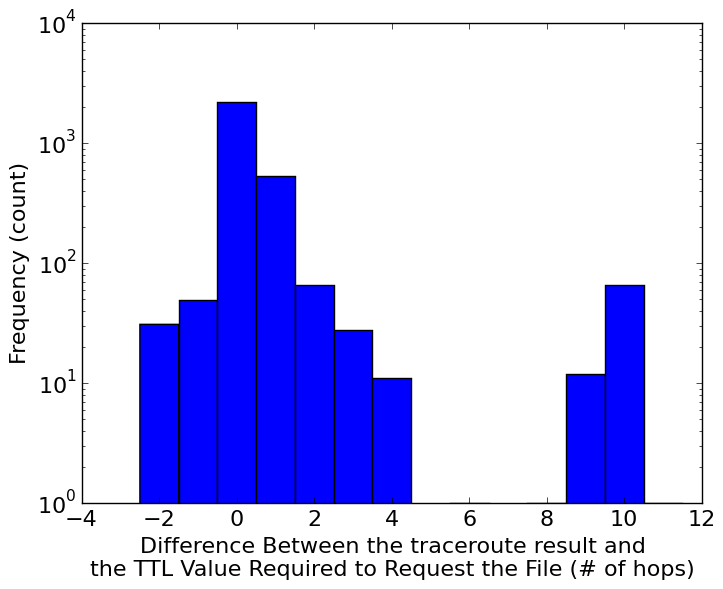
\includegraphics[width=\columnwidth]{figures/histhomepages}
	\caption{
		A histogram showing how often a file request succeeded with a TTL value less than the number of hops to the server (as estimated by the \texttt{scapy-python3}~\cite{Dobelis2015} traceroute), when downloading files from URIs scraped by the homepage-only crawler.
		A zero value on the x-axis represents files which were not received until the TTL value of the request was set to the result of the traceroute.
		Larger values on the x-axis represent files which were received when the TTL value of the request was less than the result of the traceroute.
		Negative values represent files which were not received until the TTL value of the request was set to be greater than the result of the traceroute.
		Files which were not received even when the request was sent with a TTL value 3 greater than the traceroute result are not shown.
	}
	\label{fig_histhomepages}
\end{figure}

Another probe is in progress on the partial list of 0.9 million (referer, URI) pairs generated by the full-site crawler described in \autoref{full-crawler}.
Through 20 hours, 15,662 files have been probed.
A histogram of the differences between the traceroute result for the serving domain and the minimum TTL value required to obtain each file is shown in Figure~\ref{fig_histmemfail}.
\begin{figure}
	\includegraphics[width=\columnwidth]{figures/histmemfail}
	\caption{
		A histogram showing how often a file request succeeded with a TTL value less than the number of hops to the server (as estimated by the \texttt{scapy-python3} traceroute), when downloading files from URIs scraped by the full-site crawler prior to failure in DFO mode.
	}
	\label{fig_histmemfail}
\end{figure}